\chapter[\textsc{F. Hirzebruch} and \textsc{K. J\"anich~:} Involutions and Singularities]{INVOLUTIONS AND SINGULARITIES}\label{art11}

\begin{center}
{\em By}~~ F. Hirzebruch and K. J\"anich\footnote{Presented by F. Hirzebruch}

\bigskip

{\em Heinrich Behnke zum {\rm 70.} Geburtstag gewidmet.}
\end{center}

\setcounter{pageoriginal}{218}
\section{Introduction.}\label{art11-sec1}\pageoriginale

\lhead[\thepage]{\textit{Involutions and Singularities}}
\rhead[\textit{F. Hirzebruch and K. J\"anich}]{\thepage}

Let $X$ be a compact oriented differentiable manifold without boundary of dimension $4k-1$ with $k\geq 1$. Let $T:X\to X$ be an orientation preserving fixed point free differentiable involution. In \cite{art11-key7} an invariant $\alpha(X,T)$ was defined using a special case of the Atiyah-Bott-Singer fixed point theorem. If the disjoint union $mX$ of $m$ copies of $X$ bounds a $4k$-dimensional compact oriented differentiable manifold $N$ in such a way that $T$ can be extended to an orientation preserving involution $T_{1}$ on $N$ which may have fixed points, then
\begin{equation*}
\alpha(X,T)=\dfrac{1}{m}(\tau(N,T_{1})- \tau(\Fix T_{1}\circ \Fix T_{1})).\tag{1}\label{art11-sec1-eq1}
\end{equation*}
Here $\tau(N,T_{1})$ is the signature of the quadratic form $f_{T_{1}}$ defined over $H_{2k}(N,\bfQ)$ by
$$
f_{T_{1}}(x,y)=x\circ T_{1}y
$$
where ``$\circ$'' denotes the intersection number. $\tau(\Fix T_{1}\circ \Fix T_{1})$ is the signature of the ``oriented self-intersection cobordism class'' $\Fix T_{1}\circ \Fix T_{1}$. According to Burdick \cite{art11-key4} there exist $N$ and $T_{1}$ with $m=2$.

In \S\ref{art11-sec2} we shall study a compact oriented manifold $\mathscr{D}$ whose boundary is $X-2(X/T)$. This manifold $\mathscr{D}$ was first constructed by Dold \cite{art11-key5}; we give a different description of it. Namely, $\mathscr{D}$ is a branched covering of degree $2$ of $(X/T)\times I$, where $I$ is the unit interval. The covering transformation is an orientation preserving involution $T_{1}$ of $\mathscr{D}$ which restricted to the boundary is $T$ on $X$ and the trivial involution on $2(X/T)$, and $\Fix T_{1}$ is the branching locus.

We show that
$$
\alpha(X,T)=\tau(\mathscr{D},T_{1})=-\tau(\mathscr{D}),
$$\pageoriginale
where $\tau(\mathscr{D})$ is the signature of the $4k$-dimensional manifold $\mathscr{D}$. Thus $\alpha(X,T)$ is always an integer. The construction of $\mathscr{D}$ is closely related to Burdick's result on the oriented bordism group of $B_{Z_{2}}$ and can in fact be used to prove it.

In \cite{art11-key7} it was claimed that if $X^{4k-1}$ is an integral homology sphere then $\tau(\mathscr{D})=\pm \beta(X,T)$, where $\beta(X,T)$ is the Browder-Livesay invariant \cite{art11-key3}. The proof was not carried through. It turns out that the definition of Browder-Livesay is also meaningful without assumptions on the homology of $X$. In \S\ref{art11-sec3} we shall prove
\begin{equation*}
\beta(X,T)=-\tau(\mathscr{D}).\tag{3}\label{art11-sec1-eq3}
\end{equation*}
By \eqref{art11-sec1-eq2}, we obtain
\begin{equation*}
\alpha(X,T)=\beta(X,T).\tag{4}\label{art11-sec1-eq4}
\end{equation*}
Looking at $\mathscr{D}$ as a branched covering of $(X/T)\times I$ has thus simplified considerably the proof of \eqref{art11-sec1-eq4} envisaged in \cite{art11-key7}.

If $a=(a_{0},a_{1},\ldots,a_{2k})\in \bfZ^{2k+1}$ with $a_{j}\geq 2$, then the affine algebraic variety
\begin{equation*}
z^{a_{0}}_{0}+z^{a_{1}}_{1}+\cdots+z^{a_{2k}}_{2k}=0\tag{5}\label{art11-sec1-eq5}
\end{equation*}
has an isolated singularity at the origin whose ``neighborhood boundary'' is the Brieskorn manifold \cite{art11-key1}
$$
\Sigma^{4k-1}_{a}\subset C^{2k+1}
$$
given by the equation \eqref{art11-sec1-eq5} and 
\begin{equation*}
\sum\limits^{2k}_{i=0}z_{i}\overline{z}_{i}=1.\tag{6}\label{art11-sec1-eq6}
\end{equation*}
If all the $a_{j}$ are odd, then $Tz=-z$ induces an orientation preserving fixed point free involution $T_{a}$ on $\Sigma_{a}$. The calculation of $\alpha(\Sigma_{a},T_{a})$ is an open problem (compare \cite{art11-key7}). This problem on isolated singularities is the justification for presenting our paper to a colloquium on algebraic geometry. In \S\ref{art11-sec4} we give the recipe for calculating $\alpha(\Sigma_{a},T_{a})$ for $k=1$ in the case where the exponents $a_{0}$, $a_{1}$, $a_{2}$ are pairwise prime and odd.

\section{The Dold construction.}\label{art11-sec2}\pageoriginale

Let $Y$ be a compact differentiable manifold without boundary and $W$ a 1-codimensional compact submanifold with boundary $\partial W$. Then, as it is well known, one can construct a double covering of $Y$, branched at $\partial W$, by taking two copies of $Y$, ``cutting'' them along $W$ and then identifying each boundary point of the cut in copy one with its opposite point in copy two. The same can be done if $Y$ is a manifold with boundary and $W$ intersects $\partial Y$ transversally in a union of connected components of $\partial W$. The covering will then be branched at $\partial W-\partial W\cap \partial Y$.

We are interested in a very special case of this general situation. Let $M$ be a compact differentiable manifold without boundary and $V$ a closed submanifold without boundary of codimension 1 in $M$. Then we define $Y=M\times [0,1]$ and $W=V\times [0,\frac{1}{2}]$.
\begin{figure}[H]
\centering
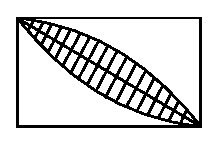
\includegraphics{src/chap11/fig1.eps}
\end{figure}

For the following we will need a detailed description of the double covering corresponding to $(M\times [0,1],V\times [0,\frac{1}{2}])$. The normal bundle of $V$ in $M$ defines a $\bfZ_{2}$-principal bundle $\widetilde{V}$ over $V$. If we ``cut'' $M$ along $V$, we obtain a compact differentiable manifold $C$ with boundary $\partial C=\widetilde{V}$. As a set, $C$ is the disjoint union of $M-V$ and $\widetilde{V}$, and there is an obvious canonical way to introduce topology and differentiable structure in $(M-V)\cup \widetilde{V}$. Similarly, let $C'$ be the disjoint union of $M\times [0,1]-V\times [0,\frac{1}{2})$ and $\widetilde{V}\times [0,\frac{1}{2})$, topologized in the canonical way. Then we consider two copies $C'_{1}$ and $C'_{2}$ of $C'$ and identify in their disjoint union each $x\in V\times \{\frac{1}{2}\}\subset C'_{1}$ with the corresponding point $x\in V\times \{\frac{1}{2}\}\subset C'_{2}$ and for $0\leq t<\frac{1}{2}$ each point $v\in \widetilde{V}\times \{t\}\subset C'_{1}$ with the opposite point $-v\in \widetilde{V}\times \{t\}\subset C'_{2}$. Let $\mathscr{D}$ denote\pageoriginale the resulting topological space and $\pi:\mathscr{D}\to M\times [0,1]$ the projection. Then $C'_{1}$, $C'_{2}$ and $V\times \{\frac{1}{2}\}$ are subspaces, and $\mathscr{D}-V\times \{\frac{1}{2}\}$ has a canonical structure as a differentiable manifold with boundary.

To introduce a differentiable structure on all of $\mathscr{D}$, we use a tubular neighbourhood of $V$ in $M$. This may be given as a diffeomorphism
$$
\kappa : \fprod{\widetilde{V}}{D^{1}}{Z_{2}}\to M
$$
onto a closed neighbourhood of $V$ in $M$, such that the restriction of $\kappa$ to $\fprod{\widetilde{V}}{\{0\}}{Z_{2}}=V$ is the inclusion $V\subset M$. Let $Z_{2}$ act on $D^{2}\subset \bfC$ by complex conjugation. Then we get a tubular neighbourhood of $V\times \{\frac{1}{2}\}$ in $M\times [0,1]$
\begin{equation*}
\begin{split}
&\lambda : \fprod{\widetilde{V}}{D^{2}}{Z_{2}}\to M\times [0,1]\quad\text{by}\\
&[v,x+iy]\mapsto (\kappa(v,y),\frac{1}{2}+\frac{1}{4}x).
\end{split}\tag{1}
\label{art11-sec2-eq1}
\end{equation*}
Let the ``projectin'' $p:\fprod{\widetilde{V}}{D^{2}}{Z_{2}}\to \fprod{\widetilde{V}}{D^{2}}{Z_{2}}$ be given on each fibre by $z\to z^{2}/|z|$. Then $\lambda p$ can be lifted to $\mathscr{D}$, which means that we can choose a map $\lambda_{1}:\fprod{\widetilde{V}}{D^{2}}{Z_{2}}\to \mathscr{D}$ such that
\begin{equation*}
\vcenter{\xymatrix{
\fprod{\widetilde{V}}{D^{2}}{Z_{2}}\ar[d]^-{p}\ar[r]^-{\lambda_{1}} & \mathscr{D}\ar[d]^-{\pi}\\
\fprod{\widetilde{V}}{D^{2}}{Z_{2}}\ar[r]^-{\lambda} & M\times [0,1]
}}\tag{2}\label{art11-sec2-eq2}
\end{equation*}
is commutative. Then there is exactly one differentiable structure on $\mathscr{D}$ for which $\lambda_{1}$ is a diffeomorphism onto a neighborhood of $V\times \{\frac{1}{2}\}$ in $\mathscr{D}$ and which coincides on $\mathscr{D}-V\times \{\frac{1}{2}\}$ with the canonical structure. Up to diffeomorphism, of course, this structure does not depend on $\kappa$.

$\mathscr{D}$, then, is a double covering of $M\times [0,1]$, branched at $V\times \{\frac{1}{2}\}$. The covering transformation on $\mathscr{D}$ shall be denoted by $T_{1}$. Note that on $\fprod{\widetilde{V}}{D^{2}}{Z_{2}}$ (identified by $\lambda_{1}$ with a subset of $\mathscr{D}$) the transformation $T_{1}$ is given by $[v,z]\to [v,-z]$.

As a differentiable manifold, $\mathscr{D}$ is the same as the manifold constructed by Dold in his note \cite{art11-key5}.

Now\pageoriginale consider once more the differentiable manifold $C$ with boundary $\partial C=\widetilde{V}$, which we obtained from $M$ by cutting along $V$. Let $C_{1}\cup C_{2}$ be the disjoint union of two copies of $C$. If we identify $x\in \widetilde{V}_{1}\subset C_{1}$ with $-x\in \widetilde{V}_{1}\subset C_{1}$ and $x\in \widetilde{V}_{2}$ with $-x\in \widetilde{V}_{2}$, we obtain from $C_{1}\cup C_{2}$ the disjoint union of two copies of $M$ :
\begin{figure}[H]
\centering
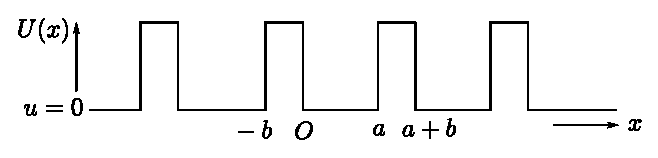
\includegraphics{src/chap11/fig2.eps}
\end{figure}
If we identify $x\in \widetilde{V}_{1}\subset C_{1}$ with $-x\in \widetilde{V}_{2}\subset C_{2}$, we get a differentiable manifold which we denote by $\widetilde{M}$ :
\begin{figure}[H]
\centering
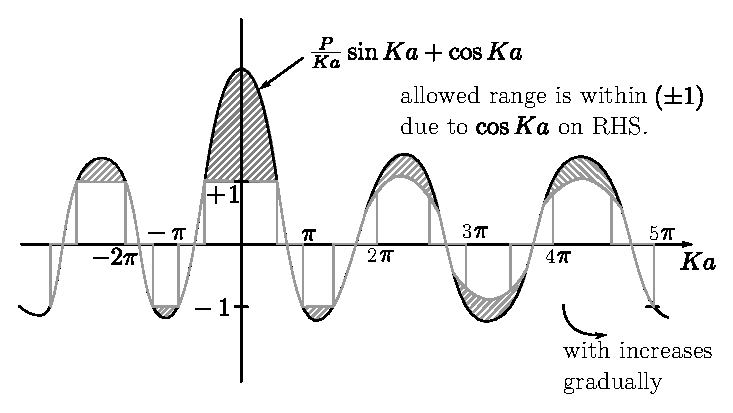
\includegraphics{src/chap11/fig3.eps}
\end{figure}
If we identify $x\in \widetilde{V}_{1}\subset C_{1}$ with $x\in \widetilde{V}_{2}\subset C_{2}$, then $C_{1}\cup C_{2}$ becomes a closed manifold $B$ (the usual ``double'' of $C$), and we use $\kappa$ to introduce the differentiable structure on $B$ :
\begin{figure}[H]
\centering
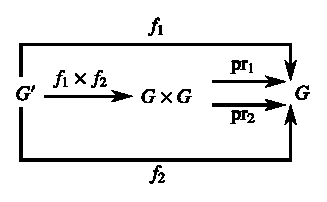
\includegraphics{src/chap11/fig4.eps}
\end{figure}
If we, finally, identify for each $x\in \widetilde{V}$ all four points $x\in \widetilde{V}_{1}$, $-x\in \widetilde{V}_{1}$, $x\in \widetilde{V}_{2}$, $-x\in \widetilde{V}_{2}$ to one, then we obtain a topological space $A$ :
\begin{equation*}
\begin{array}{c}
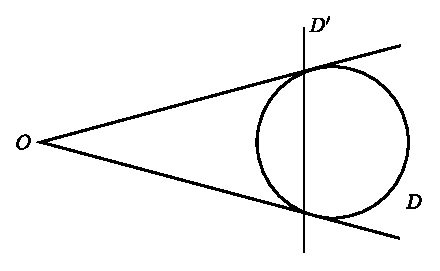
\includegraphics{src/chap11/fig5.eps}
\end{array}\tag{3}\label{art11-sec2-eq3}
\end{equation*}

Now obviously we have $2M=\pi^{1}(M\times \{1\})$, $A=\pi^{-1}(M\times \{\frac{1}{2}\})$ and $\widetilde{M}=\pi^{-1}(M\times \{0\})$, and by our choice of the differentiable structures of $B$ and $\mathscr{D}$ ($p$ in \eqref{art11-sec2-eq2} is given by $z\to z^{2}/|z|$ instead of $z\to z^{2}$), the canonical map $B\to A$ defines an {\em immersion}
$$
f:B\to \mathscr{D}.
$$
It should be mentioned, perhaps, that for the same reason $\pi:\mathscr{D}\to M\times [0,1]$ is not differentiable at $V\times \{\frac{1}{2}\}$.

Up\pageoriginale to this point, we did not make any orientability assumptions. Considering now the ``orientable case'', we shall use the following convention : for orientable manifolds with boundary, we will always choose the orientations of the manifold and its boundary in such a way, that the orientation of the boundary, followed by the inwards pointing normal vector, gives the orientation of the manifold.

Now if $X$ is any compact differentiable manifold without boundary and $T$ a fixed point free involution on $X$ with $X/T\cong M$, then $(X,T)$ is equivariantly diffeomorphic to $(\widetilde{M},T_{1}|\widetilde{M})$ for a suitably chosen $V\subset M$, and in fact our $(\widetilde{M},T_{1}|\widetilde{M})$ plays the role of the $(X,T)$ in \S\ref{art11-sec1}. Therefore we will assume from now on, that $\widetilde{M}$ is {\em oriented} and $T_{1}|\widetilde{M}$ is {\em orientation preserving}. Let us also write $T$ for $T_{1}|\widetilde{M}$.

Then the orientation of $\widetilde{M}$ defines an orientation of $M$ and hence of $C$, and since $\widetilde{V}=\partial C$, an orientation of $\widetilde{V}$ is thus determined. Furthermore, the orientation of $\widetilde{M}\subset\partial \mathscr{D}$ induces an orientation of $\mathscr{D}$, relative to which
\begin{equation*}
\partial \mathscr{D}=\widetilde{M}-2M.\tag{4}\label{art11-sec2-eq4}
\end{equation*}
Clearly $T_{1}$ on $\mathscr{D}$ is orientation preserving, $V$ may not be orientable, and $\widetilde{V}\to V$ is the orientation covering of $V$, because $M$ is orientable.

The relation of the construction of $\mathscr{D}$ to the result of Burdick is the following. Let $\Omega_{*}(\bfZ_{2})$ denote the bordism group of oriented manifolds with fixed point free orientation preserving involutions. Then we have homomorphisms
$$
\Omega_{n}\oplus \mathfrak{N}_{n-1}~{\displaystyle{\mathop{\leftrightarrows}_{j}^{i}}}~ \Omega_{n}(\bfZ_{2})
$$
as follows: if $[M]\in \Omega_{n}$ is represented by an oriented $n$-dimensional manifold $M$, the $i[M]\in \Omega_{n}(Z_{2})$ is simply given by $2M$ with the trivial involution. Now let $[W]_{2}\in \mathfrak{N}_{n-1}$ be represented by an $(n-1)$-dimensional manifold $W$, let $\widetilde{W}\to W$ denote the orientation covering, and let $Y$ be the sphere bundle of the Whitney sum of the real line bundle over $W$ associated to $\widetilde{W}$ and the trivial line bundle $W\times \bfR$:
\begin{figure}[H]
\centering
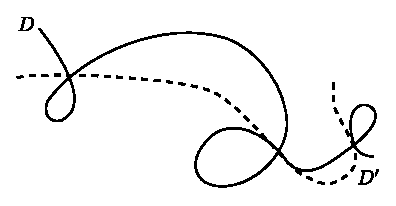
\includegraphics{src/chap11/fig6.eps}
\end{figure}\pageoriginale
\noindent
The manifold $Y$ is orientable, and we may orient $Y$ at $\widetilde{W}$ by the canonical orientation of $\widetilde{W}$ followed by the normal vector pointing toward $W\times \{1\}$. Then we denote by $i(W)$ the oriented double covering of $Y$ corresponding to $(Y,W\times \{1\})$, and we define $i[W]\in \Omega_{n}(\bfZ_{2})$ to be represented by $i(W)$.

As already mentioned, any element of $\Omega_{n}(\bfZ_{2})$ can be represented by the (unbranched) double covering $\widetilde{M}$ corresponding to some $(M,V)$, and we define $j[\widetilde{W},T]=[M]\oplus [V]_{2}$. Then $i$ and $j$ are well defined homomorphisms and clearly $j\circ i=\text{Id}$, so $i$ is injective. To show that $i$ is also surjective, we have to construct for given $(M,V)$ and $(n+1)$-dimensional oriented manifold $\mathscr{B}$ with boundary and with an orientation preserving fixed point free involution, such that equivariantly $\partial \mathscr{B}=\widetilde{M}-2M-i(V)$. But such a manifold is given by $\mathscr{B}=\pi^{-1}(M\times [0,1]-U)$,
\begin{figure}[H]
\centering
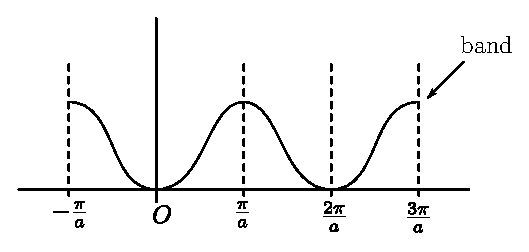
\includegraphics{src/chap11/fig7.eps}
\end{figure}
\noindent
where $U$ is the interior of the tubular neighborhood \eqref{art11-sec2-eq1} of $V\times \{\frac{1}{2}\}$ in $M\times [0,1$ :
\begin{align*}
\partial \mathscr{B} &= \pi^{-1}(M\times \{0\})\cup \pi^{-1}(M\times \{1\})\cup \pi^{-1}(\overdot{U})\\[3pt]
&= \widetilde{M}-2M-i(V).
\end{align*}
Thus\pageoriginale $i:\Omega_{n}\oplus \mathfrak{N}_{n-1}\to \Omega_{n}(\bfZ_{2})$ is an isomorphism. Brudick uses in \cite{art11-key4} essentially the same manifold $\mathscr{B}$ to prove the surjectivity of $i$.

We will now consider the invariant $\alpha$ and therefore assume that $\dim \widetilde{M}=4k-1$ with $k\geq 1$. First we remark, that for the trivial involution $T$ on $2M$ the invariant $\alpha$ vanishes: since the nontrivial elements of $\Omega_{4k-1}$ are all of order two, there is an oriented $X$ with $\partial X=2M$. Let $T'$ be the trivial involution on $2X$. Then $2\alpha(2M,T)=\tau(2X,T')=0$, because it is the signature of a quadratic form which can be given by a matrix of the form
\begin{center}
\tabcolsep=.5cm
\renewcommand{\arraystretch}{2}
\begin{tabular}{|c|c|}
\hline
$O$ & $E$\\
\hline
$E$ & $O$\\
\hline
\end{tabular}
\end{center}
where $E$ is a symmetric matrix. Hence it follows, that $\alpha(\partial \mathscr{D},T_{1}|\partial \mathscr{D})=\alpha(\widetilde{M},T)$ and therefore by \eqref{art11-sec2-eq1} of \S\ref{art11-sec1} we have
\begin{equation*}
\alpha(\widetilde{M},T)=\tau(\mathscr{D},T_{1})-\tau(\Fix T_{1}\circ \Fix T_{1}).\tag{5}\label{art11-sec2-eq5}
\end{equation*}
Notice that here we apply the definition \eqref{art11-sec1-eq1} of \S\ref{art11-sec1} of $\alpha$ in a case, where $\Fix T_{1}$ is not necessarily orientable, so that we have to use the Atiyah-Bott-Singer fixed point theorem also for the case of non-orientable fixed point sets.

\begin{prop*}
$\alpha(\widetilde{M},T)=\tau(\mathscr{D},T_{1})=-\tau(\mathscr{D})$.
\end{prop*}

\begin{proof}
$\Fix T_{1}\circ \Fix T_{1}=0\in \Omega_{*}$, since the normal bundle of $\Fix T_{1}=V\times \{\frac{1}{2}\}$ in $\mathscr{D}$ has a one-dimensional trivial subbundle. Therefore by \eqref{art11-sec2-eq5}, $\alpha(\widetilde{M},T)=\tau(\mathscr{D},T_{1})$. To show that $\tau(\mathscr{D},T_{1})=-\tau(\mathscr{D})$, let again $U$ denote our open tubular neighbourhood of $V\times \{\frac{1}{2}\}$ in $M\times [0,1]$, $\overline{U}$ its closure in $M\times [0,1]$ and correspondingly $U_{1}=\pi^{-1}(U)$, $\overline{U}_{1}=\pi^{-1}(\overline{U})$. Then $\tau(\overline{U})=\tau(\overline{U}_{1})=\tau(\overline{U}_{1},T_{1})=0$, because $\overline{U}$ and $\overline{U}_{1}$ are disc bundles of vector bundles with a trivial summand and hence the zero section, which carries all the homology, can be deformed into a section which is everywhere different from zero. Because\pageoriginale of the additivity of the signature (compare (8) of \cite{art11-key7}), we therefore have
$$
\tau(\mathscr{D},T_{1})=\tau(\mathscr{D}-U_{1},T_{1}).
$$
But $T_{1}$ is fixed point free on $\mathscr{D}-U_{1}$, and hence we can apply formula (7) of \cite{art11-key7}, which is easy to prove and which relates the signature $\tau(M^{4k},T)$ of a fixed point free involution with the signatures of $M^{4k}$ and $M^{4k}/T$ and we obtain
\begin{align*}
\tau(\mathscr{D},T_{1})=\tau(\mathscr{D}-U_{1},T_{1}) &= 2\tau(M\times [0,1]-U)-\tau(\mathscr{D}-U_{1})\\[3pt]
&= 2\tau(M\times [0,1])-\tau(\mathscr{D}).
\end{align*}
\end{proof}

\section{The Browder-Liversay invariant.}\label{art11-sec3}

The involution on $\widetilde{V}$ which is given by $x\to-x$ shall also be denoted by $T$, because it is the restriction of $T$ on $\widetilde{M}$ to $\widetilde{V}$, if we regard $\widetilde{V}$ via $\widetilde{V}_{1}\subset C_{1}\subset \widetilde{M}$ as a submanifold of $\widetilde{M}$. $T$ is orientation reversing on $\widetilde{V}$, and since the intersection form $(x,y)\to x\circ y$ on $H_{2k-1}(\widetilde{V},\bfQ)$ is skew-symmetric, the quadratic form $(x,y)\to x\circ Ty$ is symmetric on $H_{2k-1}(\widetilde{V},\bfQ)$. Now we restrict this form to
\begin{equation*}
L=\text{kernel of } H_{2k-1}(\widetilde{V},\bfQ)\to H_{2k-1}(C,\bfQ),\tag{1}\label{art11-sec3-eq1}
\end{equation*}
where the homomorphism is induced by the inclusion $\widetilde{V}=\partial C\subset C$, and we denote by $\beta(\widetilde{M},\widetilde{V},T)$ the signature of this quadratic form on $L$. (If $\widetilde{M}=\Sigma^{4k-1}$ is a homotopy sphere, then $\beta(\widetilde{M},\widetilde{V},T)$ is by definition the {\em Browder-Livesay invariant} \cite{art11-key3} $\sigma(\Sigma^{4k-1},T)$ of the involution $T$ on $\Sigma^{4k-1}$).

\begin{theorem*}
$\alpha(\widetilde{M},T)=\beta(\widetilde{M},\widetilde{V},T)$.

Thus $\beta(\widetilde{M},T)=\beta(\widetilde{M},\widetilde{V},T)$ is a well defined invariant of the oriented equivariant diffeomorphism class of $(\widetilde{M},T)$.
\end{theorem*}

\noindent
{\bf Proof of the Theorem.}~ First notice, that the canonical deformation retraction of $M\times [0,1]$ to $M\times \{\frac{1}{2}\}$ induces a deformation retraction of $\mathscr{D}=\pi^{-1}(M\times [0,1])$ to $A=\pi^{-1}(M\times \{\frac{1}{2}\})$. To study $H_{2k}(A,Q)$, we consider the following part of a Mayer-Vietoris sequence for $A$ (all homology with coefficients in $Q$): $H_{2k}(V)\oplus H_{2k}(C_{1}\cup C_{2})\xrightarrow{\phi}H_{2k}(A)\xrightarrow{\chi}$\pageoriginale
$$
H_{2k-1}(\widetilde{V}_{1}\cup \widetilde{V}_{2})\xrightarrow{\psi}H_{2k-1}(V)\oplus H_{2k-1}(C_{1}\cup C_{2})
$$
where $\widetilde{V}_{1}\cup \widetilde{V}_{2}$ and $C_{1}\cup C_{2}$ denote the disjoint unions, see figure \eqref{art11-sec2-eq3} of \S\ref{art11-sec2}.

In $H_{2k}(A)$ we have to consider the quadratic forms given by $(x,y)\to x\circ y$ and $(x,y)\to x\circ Ty$, where $\circ$ denotes the intersection number in $\mathscr{D}$. Now, the maps $V=V\times \{\frac{1}{2}\}\subset A$ and $C_{1}\cup C_{2}\to A$, which induce the homomorphism $\phi$, are homotopic in $\mathscr{D}$ to maps into $\mathscr{D}-A$. Therefore if $x\in \text{Im~}\phi\subset H_{2k}(A)$ and $y$ is any element of $H_{2k}(A)$, then $x\circ y=0$. Thus if we denote
\begin{equation*}
L'=H_{2k}(A)/\text{Im~}\phi,\tag{2}\label{art11-sec3-eq2}
\end{equation*}
then the quadratic forms $(x,y)\to x\circ y$ and $(x,y)\to x\circ Ty$ are well defined on $L'$, and their signatures as forms on $L'$ are $\tau(\mathscr{D})$ and $\tau(\mathscr{D},T_{1})$ respectively.

$L'$ is isomorphic to the kernel of $\psi$, and hence we shall now take a closer look at $\ker \psi$. For this purpose we consider the Mayer-Vietoris sequences for $\widetilde{M}$ and $B$:
\begin{align*}
& H_{2k}(\widetilde{M})\xrightarrow{\widetilde{\chi}}H_{2k-1}(\widetilde{V}_{1}\cup \widetilde{V}_{2})\xrightarrow{\widetilde{\psi}}H_{2k-1}(\widetilde{V})\oplus H_{2k-1}(C_{1}\cup C_{2})\\[4pt]
& H_{2k}(B)\xrightarrow{\chi^{B}}H_{2k-1}(\widetilde{V}_{1}\cup \widetilde{V}_{2})\xrightarrow{\psi^{B}}H_{2k-1}(\widetilde{V})\oplus H_{2k-1}(C_{1}\cup C_{2}).
\end{align*}
In the sequence for $\widetilde{M}$, the homomorphism $H_{2k-1}(\widetilde{V}_{1}\cup \widetilde{V}_{2})\to H_{2k-1}(\widetilde{V})$ is induced by the identity $\widetilde{V}_{1}\to \widetilde{V}$ on $\widetilde{V}_{1}$ and by the involution $T:\widetilde{V}_{2}\to \widetilde{V}$ on $\widetilde{V}_{2}$, in the sequence for $B$ however by the identity on both components. If we write $H_{2k-1}(\widetilde{V}_{1}\cup \widetilde{V}_{2})$ as $H_{2k-1}(\widetilde{V})\oplus H_{2k-1}(\widetilde{V})$, the kernel of $H_{2k-1}(\widetilde{V}_{1}\cup \widetilde{V}_{2})\to H_{2k-1}(C_{1}\cup C_{2})$ is $L\oplus L$, and so we get:
\begin{align*}
&\ker \widetilde{\psi}=\{(a,b)\in L\oplus L | a+Tb=0\},\\
&\ker \psi^{B}=\{(a,b)\in L\oplus L | a+b=0\}.
\end{align*}
Let\pageoriginale $a$ be an element of $H_{*}(\widetilde{V},\bfQ)$. Then $a+Ta$ vanishes if and only if $a$ is in the kernel of $H_{*}(\widetilde{V},\bfQ)\to H_{*}(V,\bfQ)$. Thus the kernel of $\psi$ is
$$
\ker \psi=\{(a,b)\in L\oplus L |a+Ta+b+Tb=0\}.
$$
$\ker \psi^{B}$ and $\ker \widetilde{\psi}$ are subspaces of $\ker \psi$, and if we write $(a,b)$ as 
$$
\left(\dfrac{a-b}{2},\dfrac{b-a}{2}\right)+\left(\dfrac{a+b}{2},\dfrac{a+b}{2}\right),
$$ 
we see that in fact
\begin{equation*}
\ker \psi = \ker \psi^{B}+\ker \widetilde{\psi}.\tag{3}\label{art11-sec3-eq3}
\end{equation*}
By the isomorphism $L'\cong \ker \psi$, which is induced by $\chi$, \eqref{art11-sec3-eq3} becomes
$$
L'=L^{B}+\widetilde{L},
$$
where $L^{B}$ denotes the subspace of $L'$ corresponding to $\ker \psi^{B}$ under this isomorphism, and $\widetilde{L}$ corresponds to $\ker \widetilde{\psi}$.

Let us first consider $\widetilde{L}$. Any element in $\widetilde{L}$ can be represented by an element $\widetilde{f}_{*}(x)$, where $x\in H_{2k}(\widetilde{M})$ and $\widetilde{f}:\widetilde{M}\to A$ is the canonical map:
\[
\xymatrix@R=1.5cm{
H_{2k}(\widetilde{M})\ar[d]^-{\widetilde{f}_{*}}\ar[r]^-{\widetilde{\chi}} & H_{2k-1}(\widetilde{V}_{1}\cup \widetilde{V}_{2})\ar[d]^-{\text{Id}}\ar[r]^-{\widetilde{\psi}} & H_{2k-1}(\widetilde{V})\oplus H_{2k-1}(C_{1}\cup C_{2})\ar[d]\\
H_{2k}(A)\ar[r]^-{\chi} & H_{2k-1}(\widetilde{V}_{1}\cup \widetilde{V}_{2})\ar[r]^-{\psi} & H_{2k-1}(V)\oplus H_{2k-1}(C_{1}\cup C_{2}).
}
\]

\smallskip

But $\widetilde{f}$ is homotopic in $\mathscr{D}$ to the inclusion $\widetilde{M}=\pi^{-1}(M\times \{0\})\subset \mathscr{D}$, hence we have $L^{B}\circ L'=0$. Therefore the quadratic forms on $L'$ given by $(x,y)\to x\circ y$ and $(x,y)\to x\circ Ty$ can be restricted to $L^{B}$ and their signatures will still be $\tau(\mathscr{D})$ and $\tau(\mathscr{D},T_{1})$.

\smallskip

Now, any element in $L^{B}\subset H_{2k}(A)/\text{Im~}\phi$ can be represented by an element $f^{B}_{*}(x)$, where $x\in H_{2k}(B)$ and $f^{B}:B\to A$ is the canonical map. Furthermore, $\chi$ induces an isomorphism between $L^{B}$ and the ``Browder-Livesay Module'' $L$, because
$$
L^{B}\xrightarrow[\cong]{} \ker \psi^{B}=\{(a,-a) | a\in L\}\cong L.
$$
Hence\pageoriginale in view of the proposition in \S\ref{art11-sec2}, out theorem would be proved if we can show that the following lemma is true.

\begin{lemma*}
Let $x$, $y\in H_{2k}(B)$ and $\overline{x}=f_{*}(x)$, $\overline{y}=f_{*}(y)$ the corresponding element under the homomorphism $f_{*}:H_{2k}(B)\to H_{2k}(\mathscr{D})$ induced by the canonical map $f:B\to A\subset \mathscr{D}$. By \eqref{art11-sec3-eq3}, we have $\chi^{B}(x)=\chi(\overline{x})=(a,-a)$ and $\chi^{B}(y)=\chi(\overline{y})=(b,-b)$ for some $a$, $b\in L$. We claim:
\begin{equation*}
-\overline{x}\circ \overline{y}=a\circ Tb\tag{4}\label{art11-sec3-eq4}
\end{equation*}
\end{lemma*}

\noindent
{\bf Proof of the Lemma.}~ First we note that we can make some simplifying assumptions on $x$ and $y$. By a theorem of Thom (\cite{art11-key9}, p. 55), up to multiplication by an integer $\neq 0$, any integral homology class of a differentiable manifold can be realized by an oriented submanifold, and hence we may assume that $x$ and $y$ are given by oriented $2k$-dimensional submanifolds of $B$, which we will again denote by $x$ and $y$. Of course $x$ and $y$ may be assumed to be transversal at $\widetilde{V}\subset B$. Then $\widetilde{V}\cap x$ and $\widetilde{V}\cap y$ are differentiable $(2k-1)$-dimensional orientable submanifolds of $\widetilde{V}$. We orient $\widetilde{V}\cap x$ (and similarly $\widetilde{V}\cap y$) as the boundary of the oriented manifold $C_{1}\cap x$. Then $\widetilde{V}\cap x$ and $\widetilde{V}\cap y$ represent $a$ and $b$ in $H_{2k-1}(\widetilde{V})$,\footnote{Or $-a$ and $-b$, but we may replace $\chi$ and $\chi^{B}$ in the Mayer-Vietoris sequences for $A$ and $B$ by $-\chi$ and $-\chi^{B}$, so let us assume that they represent $a$ and $b$.} and we shall now denote $\widetilde{V}\cap x$ by $a$ and $\widetilde{V}\cap y$ by $b$.

\vskip .05cm

Since in a neighborhood of $\widetilde{V}$, $B$ is simply $\widetilde{V}\times \bfR$ and $x$ is $a\times \bfR$, it is clear that any isotopy of $a$ in $\widetilde{V}$ can be extended to an isotopy of $x$ in $B$ which is the identity outside a given neighborhood of $\widetilde{V}$ in $B$, such that $x$ remains transversal to $\widetilde{V}$ during the isotopy. Therefore we may assume that the submanifold $a$ of $\widetilde{V}$ is transversal to $b$ and $Tb$.

\vskip .05cm

There are all the preparations we have to make in $B$. Now let us immerse $B$ into $\mathscr{D}$ and thus get immersions of $x$ and $y$ into $\mathscr{D}$ which will represent $\overline{x}$ and $\overline{y}\in H_{2k}(\mathscr{D})$. To obtain transversality of these immersions however, we immerse $x$ into $\mathscr{D}$ by the standard immersion\pageoriginale $f:Bto A\subset \mathscr{D}$ and $y$ by an immersion $f':B\to \mathscr{D}$, which is different, but isotopic to $f$.

\vskip .05cm

To define $f'$, let $0<\epsilon <\frac{1}{4}$ and choose a real-valued $C^{\infty}$-function $h$ on the interval $[0,1]$ with $h(t)=t$ for $t<\frac{1}{2}\epsilon$, $h(t)=\epsilon$ for $t>\frac{1}{2}$ and $0<h(t)\leq \epsilon$ for all other $t$. Using $\kappa : \fprod{\widetilde{V}}{D^{1}}{Z_{2}}\to M$, we get a function on $\kappa (\fprod{\widetilde{V}}{D^{1}}{Z_{2}})\subset M$ by $[v,t]\to h(|t|)$, which we now extend to a function $\overline{h}$ on $M$ by defining $\overline{h}(p)=\epsilon$ for all $p\not\in \kappa (\fprod{\widetilde{V}}{D^{1}}{Z_{2}})$. Then $M\to M\times [0,1]$, given by $p\to (p,\frac{1}{2}+\overline{h}(p))$ is obviously covered by an immersion $f':B\to \mathscr{D}$ which is isotopic to $f$.

\vskip .05cm

Then in fact the immersions $f:x\to \mathscr{D}$ and $f':y\to \mathscr{D}$ are transversal to each other, and for $p\in x$, $q\in y$ we have
$$
f(p)=f'(q)\Leftrightarrow p=q\in a\cap b\text{~~ or~~ } p=Tq\in a\cap Tb.
$$

Looking now very carefully at all orientations involved, we obtain 
\begin{equation*}
-\overline{x}\circ \overline{y}=a\circ Tb+a\circ b.\tag{5}\label{art11-sec3-eq5}
\end{equation*}
\begin{figure}[H]
\centering
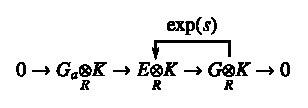
\includegraphics{src/chap11/fig8.eps}
\end{figure}

Recall that $\widetilde{V}$ is the boundary $\partial C$ of the oriented manifold $C$ and that $a$ and $b$ are in the kernel of $H_{2k-1}(\partial C)\to H_{2k-1}(C)$. Then the intersection {\em homology class} $s(a,b)\in H_{0}(\partial C)$ is in the kernel of $H_{0}(\partial C)\to H_{0}(C)$ (see Thom \cite{art11-key8}, Corollaire V.6, p. 173), and therefore the intersection {\em number} $a\circ b$ is zero, hence \eqref{art11-sec3-eq5} becomes--$\overline{x}\circ \overline{y}=a\circ Tb$, and the lemma is proved.

\section{Resolution of some singularities.}\label{art11-sec4}

For a tripel 
$$
a=(a_{0},a_{1},a_{2})
$$ 
of pairwise prime integers with $a_{j}\geq 2$ consider the variety $V_{a}\subset \bfC^{3}$ given by
\begin{equation*}
z^{a_{0}}_{0}+z^{a_{1}}_{1}+z^{a_{2}}_{2}=0.\tag{1}\label{art11-sec4-eq1}
\end{equation*}\pageoriginale
The origin is the only singularity of $V_{a}$. We shall describe a resolution of this singularity.

\begin{theorem*}
There exist a complex surface (complex manifold of complex dimension $2$) and a proper holomorphic map
$$
\phi : M_{a}\to V_{a}
$$
such that the following is true:
\begin{itemize}
\item[\rm(i)] $\phi : M_{a}-\phi^{-1}(0)\to V_{a}-\{0\}$ is biholomorphic.

\item[\rm(ii)] $\phi^{-1}(0)$ is a union of finitely many rational curves which are non-singularly imbedded in $M_{a}$.

\item[\rm(iii)] The intersection of three of these curves is always empty. Two of these curves do not intersect or intersect transversally in exactly one point.

\item[\rm(iv)] We introduce a finite graph $\mathfrak{g}_{a}$ in which the vertices correspond to the curves and in which two vertices are joined by an edge if and only if the corresponding curves intersect. $\mathfrak{g}_{a}$ is star-shaped with three rays.

\item[\rm(v)] The graph $\mathfrak{g}_{a}$ will be weighted by attaching to each vertex the self-intersection number of the corresponding curve. This number is always negative. Thus $\mathfrak{g}_{a}$ looks as follows.
\begin{figure}[H]
\centering
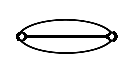
\includegraphics{src/chap11/fig9.eps}
\end{figure}

\item[\rm(vi)] $b=1$\pageoriginale or $b=2$; $b^{j}_{i}\geq 2$. Let $q_{0}$ be determined by
$$
0<q_{0}<a_{0}\quad\text{and}\quad q_{0}\equiv - a_{1}a_{2}\mod a_{0}
$$
and define $q_{1}$, $q_{2}$ correspondingly. Let $q'_{j}$ be given by
$$
0<q'_{j}<a_{j}\text{~~ and~~ } q_{j}q'_{j}\equiv 1\mod a_{j}.
$$
Then the numbers $b^{j}_{i}$ in the graph $\mathfrak{g}_{a}$ are obtained from the continued fractions
\begin{figure}[H]
\centering
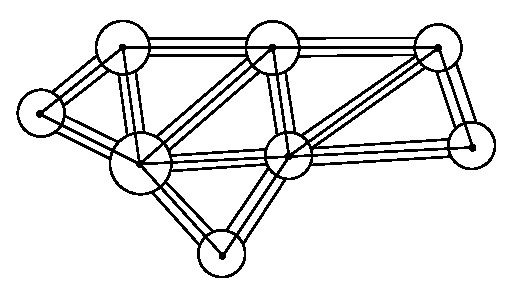
\includegraphics{src/chap11/fig10.eps}
\end{figure}

\item[\rm(vii)] If the exponents $a_{0}$, $a_{1}$, $a_{2}$ are all odd, then
\begin{align*}
& b=1\Leftarrow \Rightarrow q'_{0}+q'_{1}+q'_{2}\equiv 0\mod 2,\\[3pt]
& b=2\Leftarrow \Rightarrow q'_{0}+q'_{1}+q'_{2}\equiv 1\mod 2.
\end{align*}
\end{itemize}
\end{theorem*}

Before proving (i)-(vii) we study as an example
\begin{equation*}
z^{3}_{0}+z^{6j-1}_{1}+z^{18j-1}_{2}=0.\tag{2}\label{art11-sec4-eq2}
\end{equation*}
We have
\begin{align*}
& q_{0}=q'_{0}=2\\[3pt]
& q_{1}=4\text{~ for~ } j=1\text{~ and~ } q_{1}=6j-7\text{~ for~ } j\geq 2\\[3pt]
& q'_{1}=5j-1\\[3pt]
& q_{2}=2, q'_{2}=9j.
\end{align*}
By (vii) we get $b=2$. The continued fractions for $\dfrac{3}{2}$, $\dfrac{5}{4}$ resp. $\dfrac{6j-1}{6j-7}$, $\dfrac{18j-1}{2}$ lead then to the graph

\eject

\begin{equation}
\begin{array}{c}
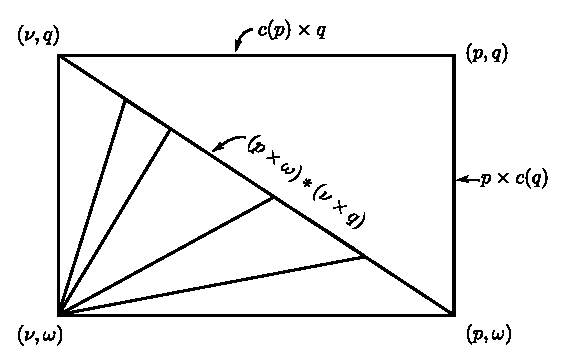
\includegraphics{src/chap11/fig11.eps}
\end{array}\label{art11-sec4-eq3}
\end{equation}\pageoriginale

\noindent
{\bf Proof of the preceding theorem.}~ We use the methods of \cite{art11-key6}. The algebroid function
$$
f=(-x_{1}^{a_{1}a_{2}}-x_{2}^{a_{1}a_{2}})^{1/a_{0}}
$$
defines a branched covering $V^{(1)}_{a}$ of $\bfC^{2}$ (coordinates $x_{1}$, $x_{2}$ in $\bfC^{2}$). Blowing up the origin of $\bfC^{2}$ (compare \cite{art11-key6}, \S1.3) gives a complex surface $W$ with a non-singular rational curve $K\subset W$ of self-intersection number $-1$ and an algebroid function $\widetilde{f}$ on $W$ branched along $K$ and along $a_{1}a_{2}$ lines which intersect $K$ in the $a_{1}a_{2}$ points of $K$ satisfying
\begin{equation*}
-x_{1}^{a_{1}a_{2}}-x_{2}^{a_{1}a_{2}}=0\tag{4}\label{art11-sec4-eq4}
\end{equation*}
where $x_{1}$, $x_{2}$ are now regarded as homogeneous coordinates of $K$. The algebroid function $\widetilde{f}$ defines a complex space $V^{(2)}_{a}$ lying branched over $W$ with $a_{1}a_{2}$ singular points lying over the points of $K$ defined by \eqref{art11-sec4-eq4}. In a neighborhood of such a point we have
\begin{equation*}
\widetilde{f}=(\zeta_{1}\zeta_{2}^{a_{1}a_{2}})^{1/a_{0}}\tag{5}\label{art11-sec4-eq5}
\end{equation*}
where $\zeta_{2}=0$ is a suitable local equation for $K$ and $\zeta_{1}=0$ for the line passing through the point and along which $V^{(2)}_{a}$ is branched over $W$.\pageoriginale The singularity of type \eqref{art11-sec4-eq5} can be resolved according to \cite{art11-key6}, \S3.4, where
\begin{equation*}
\omega=(z_{1}z_{2}^{n-q})^{1/n},\quad (0<q<n,(q,n)=1)\tag{6}\label{art11-sec4-eq6}
\end{equation*}
was studied. In our case, we have
$$
n=a_{0}\quad\text{and}\quad q=q_{0},\quad\text{see (vi) above,}
$$
for all the $a_{1}a_{2}$ singular points of $V^{(2)}_{a}$. The resolution gives a complex surface $V^{(3)}_{a}$ with the following property. The singularity of $V^{(1)}_{a}$ was blown up in a system of rational curves satisfying (iii) and represented by a star-shaped graph with $a_{1}a_{2}$ rays of the same kind. The following diagram shows only one ray where the unweighted vertex represents the central curve $\widetilde{K}$ which under the natural projection $V^{(3)}_{a}\to W$ has $K$ as bijective image
\begin{equation*}
\begin{array}{c}
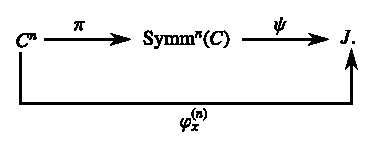
\includegraphics{src/chap11/fig12.eps}
\end{array}\tag{7}\label{art11-sec4-eq7}
\end{equation*}

$V^{(1)}_{a}$ is of course just the affine variety
$$
x^{a_{0}}_{0}+x_{1}^{a_{1}a_{2}}+x^{a_{1}a_{2}}_{2}=0
$$
which can be mapped onto $V_{a}$ (see (\eqref{art11-sec4-eq1}) by
$$
(x_{0},x_{1},x_{2})\to (z_{0},z_{1},z_{2})=(x_{0},x^{a_{2}}_{1},x^{a_{1}}_{2}).
$$
Denote by $G$ the finite group of linear transformations
\begin{equation*}
\begin{array}{c}
(x_{1},x_{2})\to (\epsilon_{2}x_{1},\epsilon_{1}x_{2})\quad\text{with}\quad \epsilon^{a_{2}}_{2}=\epsilon_{1}^{a_{1}}=1.\\
V_{a}=V^{(1)}_{a}/G.
\end{array}\tag{8}\label{art11-sec4-eq8}
\end{equation*}
Then the group $G$ operates also on $V^{(3)}_{a}$. There are two fixed points, namely the points $0=(0,1)$ and $\infty=(1,0)$ of $\widetilde{K}=K$ (with respect to the homogeneous coordinates $x_{1}$, $x_{2}$ on $K$). The $a_{1}a_{2}$ points of $\widetilde{K}$ in which the curves with self-intersection number $-b^{0}_{t_{0}}$ of the $a_{1}a_{2}$ rays intersect $\widetilde{K}$ are an orbit under $G$. The $a_{1}a_{2}$ rays are all identified in $V^{(3)}_{a}/G$. Thus $V^{(3)}_{a}/G$ is a complex space with two singular points $P_{0}$, $P_{\infty}$ corresponding to the fixed points. $V^{(3)}_{a}/G$ is thus obtained from $V_{a}$ by blowing up the singular point in a system of $t_{0}+1$ rational curves showing the following intersection behaviour:
\begin{equation*}
\begin{array}{c}
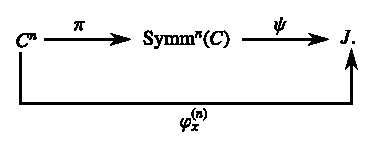
\includegraphics{src/chap11/fig12.eps}
\end{array}\tag{9}\label{art11-sec4-eq9}
\end{equation*}\pageoriginale 
but where the vertex without weight represents a rational curve passing through the singular points $P_{0}$, $P_{\infty}$.

We must find the representation of $G$ in the tangent spaces of the fixed points $0=(0,1)$ and $\infty=(1,0)$. In the neighborhood of $0$ we have local coordinates such that
\begin{equation*}
y_{1}=\dfrac{x_{1}}{x_{2}}\quad\text{and}\quad x_{2}=y^{a_{0}}_{2}.\tag{10}\label{art11-sec4-eq10}
\end{equation*}
We consider $G$ as the multiplicative group of all pairs $(\delta_{2},\delta_{1})$ with $\delta^{a_{2}}_{2}=\delta^{a_{1}}_{1}=1$ and put $\delta^{a_{0}}_{1}=\epsilon_{1}$ and $\delta_{2}=\epsilon_{2}$ (see \eqref{art11-sec4-eq8}). Then $G$ operates in the neighborhood of the fixed point $0$ as follows:
\begin{equation*}
(y_{1},y_{2})\to (\delta_{2}\delta^{-a_{0}}_{1}y_{1}, \delta_{1}y_{2}).\tag{11}\label{art11-sec4-eq11}
\end{equation*}
Thus $P_{0}$ is the quotient singularity with respect to the action \eqref{art11-sec4-eq11}. If we first take the quotient with respect to the subgroup $G_{0}$ of $G$ given by $\delta_{1}=1$ we obtain a non-singular point which admits local coordinates $(t_{1},t_{2})$ with
\begin{equation*}
t_{1}=y^{a_{2}}_{1}\quad\text{and}\quad t_{2}=y_{2}.\tag{12}\label{art11-sec4-eq12}
\end{equation*}
Thus $P_{0}$ is the quotient singularity with respect to the action of $G/G_{0}$ which is the group of $a_{1}$-th roots of unity. By \eqref{art11-sec4-eq11} and \eqref{art11-sec4-eq12} for $\delta^{a_{1}}_{1}=1$ the action is
\begin{equation*}
(t_{1},t_{2})\to (\delta^{-a_{0}a_{2}}_{1}t_{1},\delta_{1}t_{2})=(\delta^{q_{1}}_{1}t_{1},\delta_{1}t_{2}).\tag{13}\label{art11-sec4-eq13}
\end{equation*}
Looking at the invariants $\zeta_{1}=t^{a_{1}}_{1}$, $\zeta_{2}=t^{a_{1}}_{2}$ and $w=t_{1}t^{a_{1}-q_{1}}_{2}$ for which
$$
w^{a_{1}}=\zeta_{1}\zeta^{a_{1}-q_{1}}_{2}
$$
we see that $P_{0}$ is a singularity of type \eqref{art11-sec4-eq6}. We use \cite{art11-key6}, \S3.4 (or \cite{art11-key2}, Satz 2.10) for $P_{0}$ and in the same way for $P_{\infty}$ and have finished the proof except for the statements on $b$ in (vi) and (vii). The surface $M_{a}$ of the theorem is $V^{(3)}_{a}/G$ with $P_{0}$ and $P_{\infty}$ resolved. The function $f$ we started from gives rise to a holomorphic function on $M_{a}$. Using the formulas of \cite{art11-key6}, \S3.4, we see that $f$ has on the central curve of $M_{a}$ the multiplicity $a_{1}a_{2}$, and on the three curves intersecting the central curve the multiplicities 
$$
(a_{1}a_{2}q'_{0}+1)/a_{0},a_{2}q'_{1},a_{1}q'_{2}.
$$\pageoriginale
By \cite{art11-key6}, \S1.4 (1), we obtain
$$
a_{0}a_{1}a_{2}b=q'_{0}a_{1}a_{2}+q'_{1}a_{0}a_{2}+q'_{2}a_{0}a_{1}+1.
$$
Therefore
$$
a_{0}a_{1}a_{2}b<3a_{0}a_{1}a_{2}\quad\text{and}\quad b=1\quad\text{or}\quad 2.
$$
The congruence in (vii) also follows. This completes the proof.

\begin{remark*}
Originally the theorem was proved by using the $\bfC^{*}$-action on the singularity \eqref{art11-sec4-eq1} and deducing abstractly from this that the resolution must look as described. Brieskorn constructed the resolution explicitly by starting from $x^{n}_{0}+x^{n}_{1}+x^{n}_{2}(n=a_{0}a_{1}a_{2})$ and then passing to a quotient. This is more symmetric. The method used in this paper has the advantage to give the theorem also for some other equations $z^{a_{0}}_{0}+h(z_{1},z_{2})=0$ as was pointed out by Abhyankar in Bombay.
\end{remark*}

Now suppose moreover that the exponents $a_{0}$, $a_{1}$, $a_{2}$ are all odd. The explicit resolution shows that the involution $Tz=-z$ of $\bfC^{3}$ can be lifted to $M_{a}$. The lifted involution is also called $T$. It has no fixed points outside $\phi^{-1}(0)$. It carries all the rational curves of the graph $\mathfrak{g}_{a}$ over into themselves \cite{art11-key7}. Thus $T$ has the intersection points of two curves as fixed points. Let $\Fix T$ be the union of those curves which are pointwise fixed. Then $\Fix T$ is given by the following recipe.

\begin{theorem*}
For the involution $T$ on $M_{a}(a_{0},a_{1},a_{2}\text{~ odd})$ we have: The central curve belongs to $\Fix T$. If a curve is in $\Fix T$, then the curves intersecting it are not in $\Fix T$. If the curve $C$ is not in $\Fix T$ and not an end curve of one of the three rays, then the following holds: If the self-intersection number $C\circ C$ is even, then the two curves intersecting $C$ are both in $\Fix T$ or both not. If $C\circ C$ is odd, then one of the two curves intersecting $C$ is in $\Fix T$ and one not. If $C$ is an end curve of one of the three rays and if $C$ is not in $\Fix T$, then $C\circ C$ is odd if and only if the curve intersecting $C$ belongs to $\Fix T$.
\end{theorem*}

\begin{proof}
The\pageoriginale involution can be followed through the whole resolution. It is the identity on the curve $K$. On the three singularities of type \eqref{art11-sec4-eq6} the involution is given by $(z_{1},z_{2})\to (z_{1},-z_{2})$. Here $z_{1}$ and $z_{2}$ are not coordinate functions of $C^{3}$ as used in \eqref{art11-sec4-eq1}, but have the same meaning as in \cite{art11-key6}, \S3.4. The theorem now follows from formula (8) in \cite{art11-key6}, \S3.4. Compare also the lemma at the end of \S6 of \cite{art11-key7}.

For $a_{0},a_{1},a_{2}$ pairwise prime and odd, we can now calculate the invariant $\alpha$ of the involution $T_{a}$ on $\Sigma^{3}_{(a_{0},a_{1},a_{2})}$ (see the Introduction). The quadratic form of the graph $\mathfrak{g}_{a}$ is negative-definite. Therefore (\cite{art11-key7}, \S6)
\begin{equation*}
\alpha(\Sigma^{3}_{(a_{0},a_{1},a_{2})},T_{a})=-(t_{0}+t_{1}+t_{2}+1)-\Fix T\circ \Fix T.\tag{14}\label{art11-sec4-eq14}
\end{equation*}
Here $t_{0}+t_{1}+t_{2}+1$ is the number of vertices of $\mathfrak{g}_{a}$ whereas $\Fix T\circ \Fix T$ is of course the sum of the self-intersection numbers of the curves belonging to $\Fix T$. The calculation of $\alpha$ is a purely mechanical process by the two theorems of this \S. The number $\alpha$ in \eqref{art11-sec4-eq14} is always divisible by 8 (compare \cite{art11-key7}) and for $(a_{0},a_{1},a_{2})=(3,6j-1,18j-1)$ we get for $\alpha$ the value $8j$ (see \eqref{art11-sec4-eq3}).

Observe that
\begin{equation*}
\Fix T\circ C\equiv C\circ C\mod 2\tag{15}\label{art11-sec4-eq15}
\end{equation*}
for all curves in the graph $\mathfrak{g}_{a}$, a fact which is almost equivalent to our above recipe for $\Fix T$. The quadratic form of $\mathfrak{g}_{a}$ has determinant $\pm 1$ because $\Sigma^{3}_{(a_{0},a_{1},a_{2})}$ is for pairwise prime $a_{j}$ an integral homology sphere (\cite{art11-key1}, \cite{art11-key2}, \cite{art11-key7}). The divisibility of $\alpha$ by 8 is then a consequence of a well known theorem on quadratic forms.

The manifold $\Sigma^{2n-1}_{a}$ (see the Introduction) is diffeomorphic to the manifold $\Sigma^{2n-1}_{a}(\epsilon)$ given by
\begin{align*}
z^{a_{0}}_{0}+\cdots+z^{a_{n}}_{n} &=\epsilon\tag{16}\label{art11-sec4-eq16}\\
\Sigma z_{i}\overline{z}_{i} &= 1,
\end{align*}
where $\epsilon$ is sufficiently small and not zero. $\Sigma^{2n-1}_{a}(\epsilon)$ bounds the manifold $N_{a}(\epsilon)$ given by
\begin{align*}
z^{a_{0}}_{0}+\cdots+ z^{a_{n}}_{n} &=\epsilon\tag{17}\label{art11-sec4-eq17}\\
\Sigma z_{i}z_{i} &\leq 1.
\end{align*}
This\pageoriginale fact apparently cannot be used to investigate the involution $T_{a}$ in the case of odd exponents because then \eqref{art11-sec4-eq17} is not invariant under $T_{a}$. If, however, the exponents are all even, then \eqref{art11-sec4-eq17} is invariant under $T_{a}$ and for $n=2k$ the number $\alpha(\Sigma^{4k-1}_{a},T_{a})$ can be calculated using like Brieskorn \cite{art11-key1} the results of Pham on $N_{a}(\epsilon)$. We get in this way
\end{proof}

\begin{theorem*}
Let $a=(a_{0},a_{1},\ldots,a_{2k})$ with $a_{i}\equiv 0\mod 2$. Then
\begin{equation*}
\alpha (\Sigma^{4k-1}_{a},T_{a})=\sum\limits_{j}\epsilon (j)(-1)^{j_{0}+\cdots+j_{2k}}.\tag{18}\label{art11-sec4-eq18}
\end{equation*}
\end{theorem*}

The sum is over all $j=(j_{0},j_{1},\ldots,j_{2k})\in Z^{2k+1}$ with $0<j_{r}<a_{r}$ and $\epsilon(j)$ is $1$, $-1$ or $0$ depending upon whether the sum $\dfrac{j_{0}}{a_{0}}+\cdots+\dfrac{j_{2k}}{a_{2k}}$ lies strictly between $0$ and $1\mod 2$, or strictly between $1$ and $2\mod 2$, or is integral.

\begin{remark*}
For simplicity the resolution was only constructed for the exponents $a_{0}$, $a_{1}$, $a_{2}$ being pairwise relatively prime. The resolution of the singularity
$$
z^{a_{0}}_{0}+z^{a_{1}}_{1}+z^{a_{2}}_{2}=0
$$
can also be done in a similar way for arbitrary exponents and gives the following information.
\end{remark*}

\begin{theorem*}
If $a_{0}\equiv a_{1}\equiv a_{2}\mod 2$ and $d$ is any integer $\geq 1$, then
$$
\alpha(\Sigma^{3}_{(da_{0},da_{1},da_{2})},T_{da})=d\alpha(\Sigma^{3}_{(a_{0},a_{1},a_{2})},T_{a})+d-1.
$$
\end{theorem*}

For $a_{0}$, $a_{1}$, $a_{2}$ all odd and $d=2$ we get
$$
\alpha(\Sigma^{3}_{(a_{0},a_{1},a_{2})},T_{a})=\frac{1}{2}(\alpha(\Sigma^{3}_{(2a_{0},2a_{1},2a_{2})},T_{2a})-1)
$$
and therefore a method to calculate $\alpha$ also for odd exponents by formula \eqref{art11-sec4-eq18}.

\begin{thebibliography}{99}
\bibitem{art11-key1} \textsc{E. Brieskorn :}\pageoriginale Beispiele zur Differentialtopologie von Singularit\"aten, {\em Invent. Math.} 2, 1-14 (1966).

\bibitem{art11-key2} \textsc{E. Brieskorn :} Rationale Singularit\"aten komplexer Fl\"achen, {\em Invent. Math.} 4, 336-358 (1968).

\bibitem{art11-key3} \textsc{W. Browder} and \textsc{G. R. Livesay :} Fixed point free involutions on homotopy spheres, {\em Bull. Amer. Math. Soc.} 73, 242-245 (1967).

\bibitem{art11-key4} \textsc{R. O. Burdick :} On the oriented bordism groups of $\bfZ_{2}$, {\em Proc. Amer. Math. Soc.} (to appear).

\bibitem{art11-key5} \textsc{A. Dold :} D\'emonstration \'el\'ementaire de deux r\'esultats du cobordisme, {\em S\'eminaire de topologie et de g\'eom\'etrie diff\'erentielle,} dirig\'e par C. Ehresmann, Paris, Mars 1959.

\bibitem{art11-key6} \textsc{F. Hirzebruch :} \"Uber vierdimensionale Riemannsche Fl\"achen mehrdeutiger analytischer Funktionen von zwei komplexen Ver\"anderlichen, {\em Math. Ann.} 126, 1-22 (1953). 

\bibitem{art11-key7} \textsc{F. Hirzebruch :} Involutionen auf Mannigfaltigkeiten, {\em Proceedings of the Conference on Transformation Groups, New Orleans} 1967, {\em Springer-Verlag}, 148-166 (1968).

\bibitem{art11-key8} \textsc{R. Thom :} Espaces fibr\'es en sph\`eres et carr\'es de Steenrod, {\em Ann. sci. \'Ecole norm. sup.} 69 (3), 109-181 (1952).

\bibitem{art11-key9} \textsc{R. Thom :} Quelques propri\'et\'es globales des vari\'et\'es diff\'erentiables, {\em Comment. Math. Helv.} 28, 17-86 (1954).
\end{thebibliography}

\bigskip
\noindent
{\small Universit\"at Bonn.}
